\documentclass{beamer}
\usetheme{Madrid}
\usepackage[utf8]{inputenc}
\usepackage[T1]{fontenc}
\usepackage{graphicx}
\usepackage{lmodern}

% Pour enlever le \institute du bas de page
% Rapetisser les noms et date etc dans le footer
\setbeamertemplate{footline}
{
	\leavevmode%
	\hbox{%
	\begin{beamercolorbox}[wd=.333333\paperwidth,ht=2.25ex,dp=1ex,center]{author in head/foot}%
	\
	\end{beamercolorbox}%
	\begin{beamercolorbox}[wd=.333333\paperwidth,ht=2.25ex,dp=1ex,center]{title in head/foot}%
	\usebeamerfont{title in head/foot}\insertshorttitle
	\end{beamercolorbox}%
	\begin{beamercolorbox}[wd=.333333\paperwidth,ht=2.25ex,dp=1ex,right]{date in head/foot}%
	\usebeamerfont{date in head/foot}\insertshortdate{}\hspace*{2em}
	\insertframenumber{} / \inserttotalframenumber\hspace*{2ex} 
	\end{beamercolorbox}}%
	\vskip0pt%
}

\AtBeginSection[]
{
	\begin{frame}
		\tableofcontents[currentsection,hideallsubsections]
	\end{frame}
}

\title{Soutenance Projet TER}
\author{Baptiste Saleil, Geoffrey Mélia, Julien Pagès, Kevin Bollini}
\date{25 avril 2012}

\begin{document}
	\begin{frame}
		\titlepage
	\end{frame}

	%Plan
	\begin{frame}{Plan}
		\tableofcontents
	\end{frame}

	\section{Introduction}
		\begin{frame}{Introduction}
		\begin{center}
		\LARGE{Ter de Master 1 : Tableau virtuel interactif}
		\end{center}
		
		But du projet :
		\begin{itemize}
		\item Concevoir une application avec une interface naturelle (mouvements)
		\item Librairie de reconnaissance de mouvements
		\item Application pour exploiter cette librairie pour dessiner ou écrire
		\end{itemize}
		
		\end{frame}

		
	\section{Analyse et Conception}
	\subsection{Choix de conceptions}
		\begin{frame}{Choix de conceptions}
			\begin{block}{Choix principaux}
				Découper le projet en deux parties distinctes : \\
				- une librairie réutilisable \\
				- une application avec une interface naturelle exploitant cette librairie \\
			\end{block}
		\end{frame}
		
	\subsection{Gestion de projet}
		\begin{frame}{Gestion de projet}
		Organisation :
			\begin{itemize}
				\item{Réunions}
				\item{Deux sous-groupes}
				\item{Partage des tâches au sein des groupes}
				\item{Décisions communes (à quatre)}
			\end{itemize}
		
		Collaboration :
			\begin{itemize}
				\item{Gestionnaire de version (Subversion)}
				\item{Partage de documents (Mail et Subversion)}
				\item{Discussions (Mails / Instantanée)}
				\item{Édition collaborative pour le travail à distance (Gobby)}
			\end{itemize}
		\end{frame}
		
		\begin{frame}{Gestion de projet}
			Objectif :
			\begin{itemize}
			\item Se renseigner, réaliser une architecture de qualité
			\item Développer rapidement un prototype
			\item Développement incrémental en ajoutant des fonctionnalités
			\end{itemize} 
		\end{frame}
		
		\begin{frame}{Rétroplanning}	
			Rétroplanning (Diagramme de gantt) :
			\begin{center}
			% TODO : mettre à jour le rétroplanning
			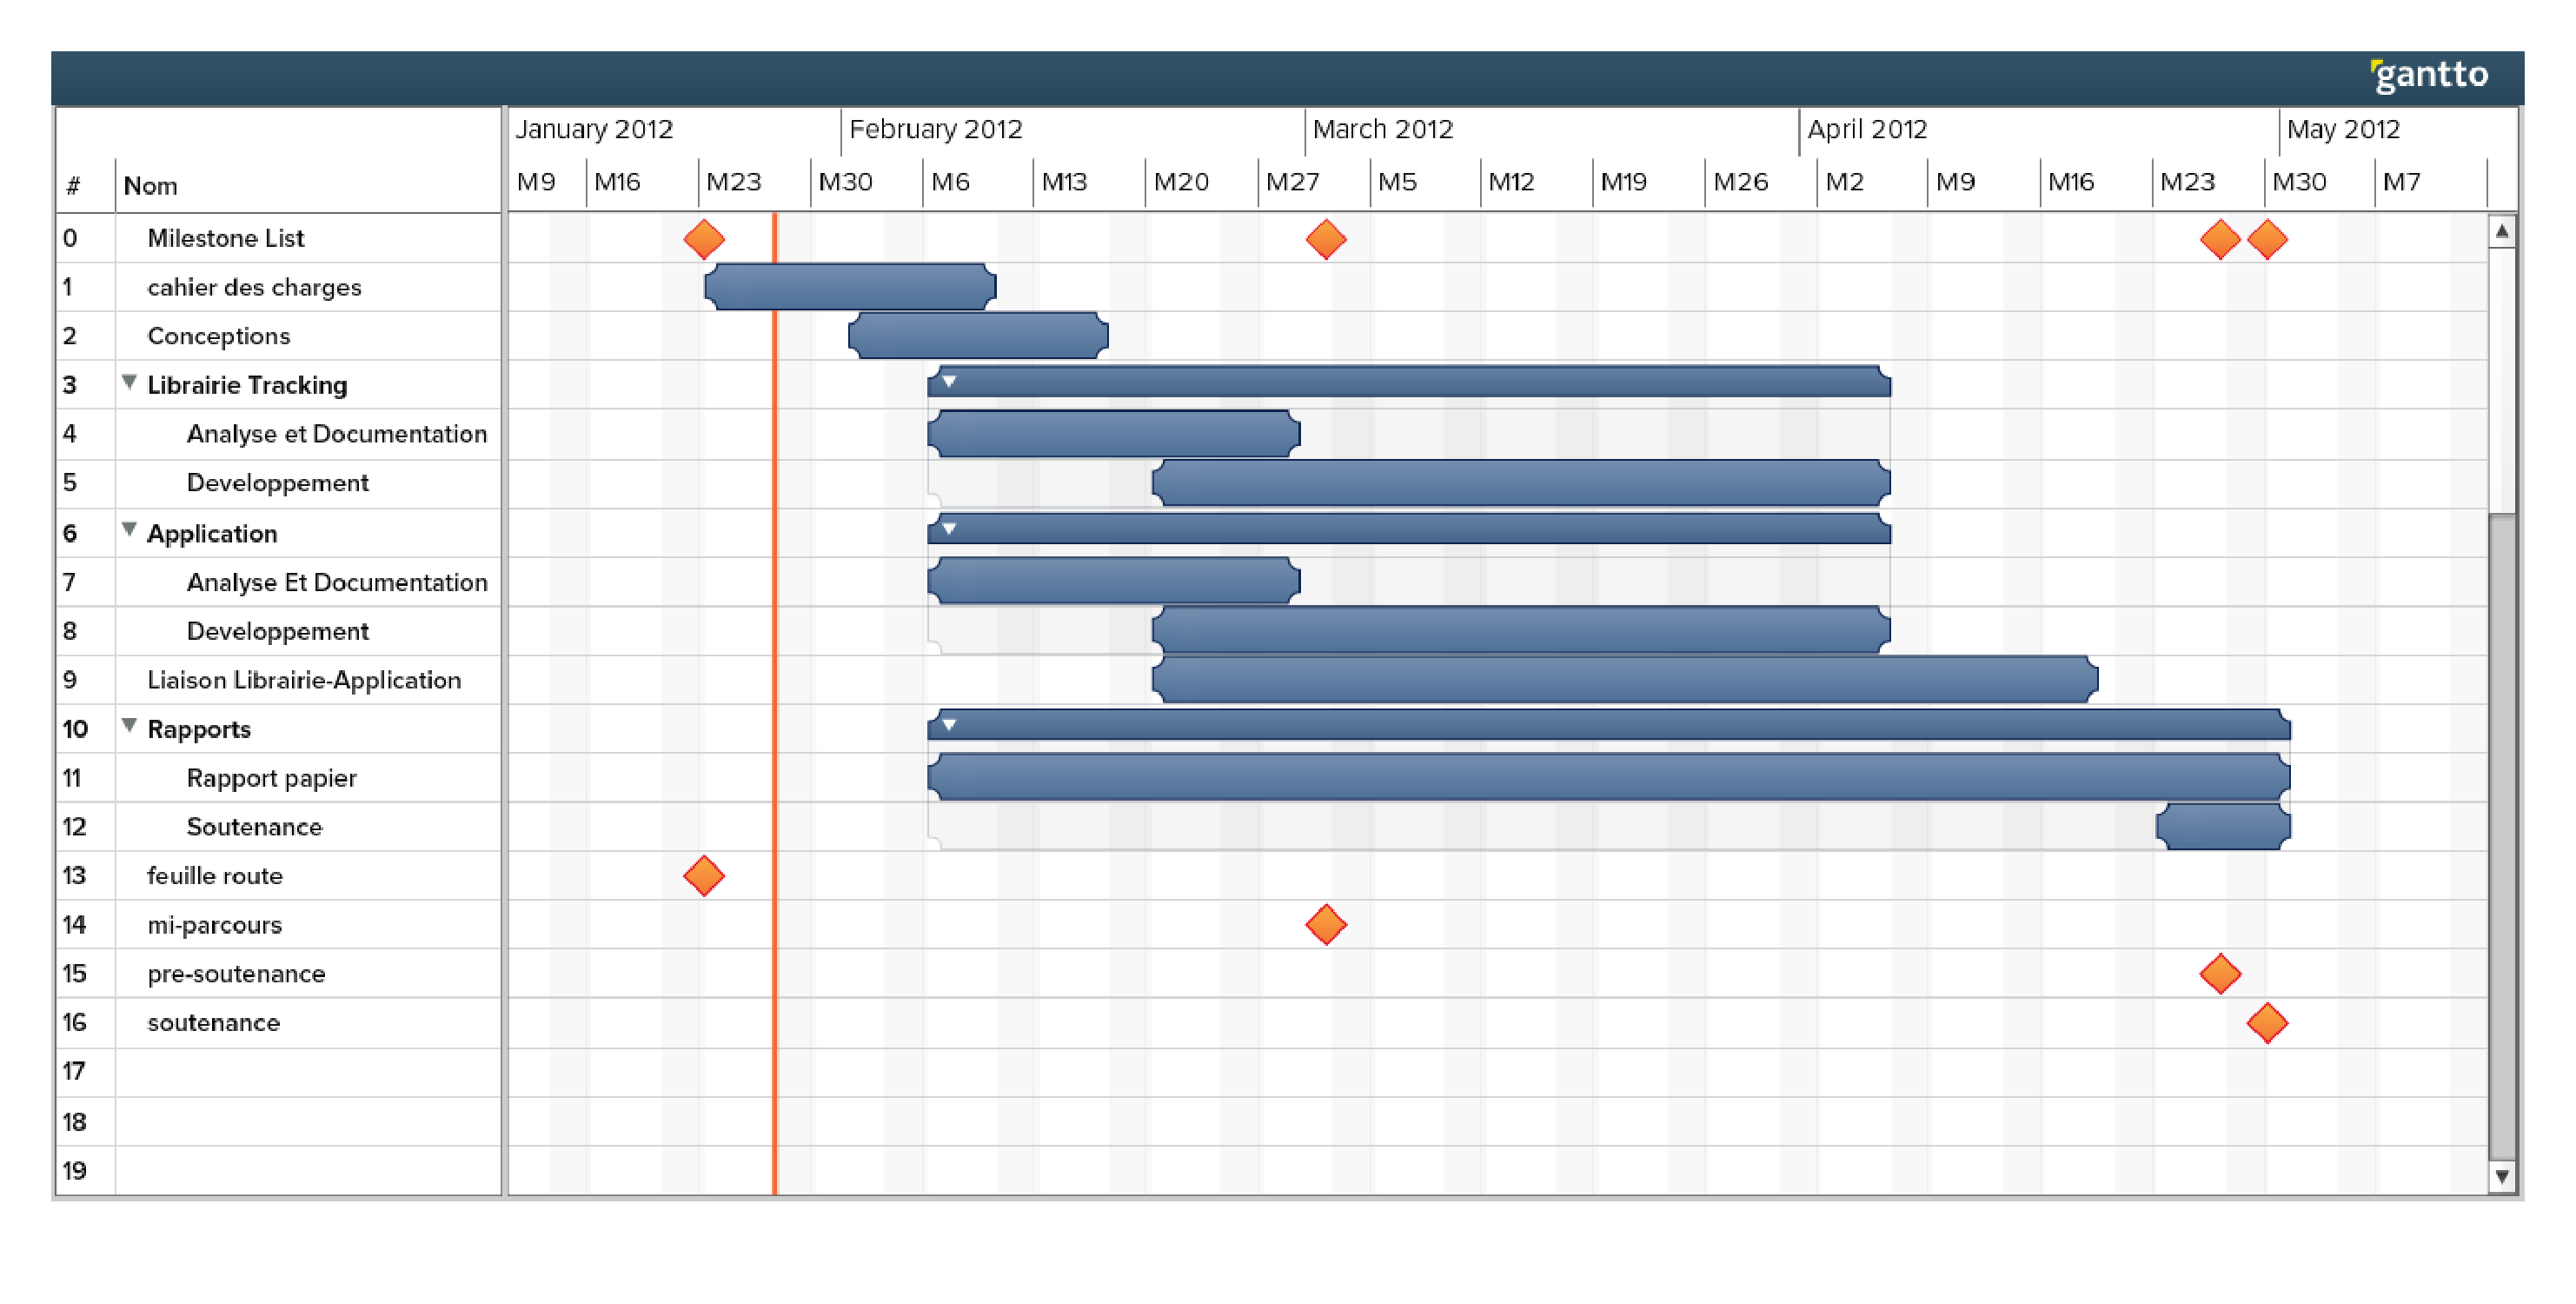
\includegraphics[scale=0.25]{../feuille-route/retroplanning.pdf}
			\end{center}
		\end{frame}
	
	\subsection{Analyse}
		\begin{frame}{Analyse}
			\begin{exampleblock}{Objectifs}
				\begin{itemize}
					\item{Identifier les besoins et envies potentiels des utilisateurs}
					\item{Distinguer et classer les fonctionnalités de l'application}
					\item{Établir un schéma de conception dans le temps}
					\item{Faciliter le développement, avoir des buts concrets}
				\end{itemize}
			\end{exampleblock}
		\end{frame}
	
	\section{Librairie}
		\begin{frame}{Librairie de suivi d'objets}
			\begin{block}{Objectifs de la librairie conçue}
				\begin{itemize}
				\item{Distinguer complètement le suivi d'objet de l'application}
				\item{Avoir une utilisation simple sans connaissance en traitement d'image}
				\item{Permettre une détection d'action}
				\item{Proposer un maximum de solutions de traçage}
				\item{Évaluer et comparer ces solutions}
				\end{itemize}
			\end{block}
		\end{frame}

		\begin{frame}{Librairie}

		Création d'une structure de données : Cursor\\
		struct Cursor \{
		\begin{itemize}
			\item{CvPoint center}
			\item{CvPoint cornerA}
			\item{CvPoint cornerB}
			\item{...}
			\item{IplImage *mask}
			\item{Bool active}
		\end{itemize}
		\} \\
		\end{frame}
		
		\begin{frame}{Librairie}
		Deux fonctions enveloppes : \\
			\begin{itemize}
				\item{Cursor * calibration(IplImage * source, CvPoint A, CvPoint B, TYPE-TRACK flag)}
				\item{int track(IplImage * source, Cursor * oldCursor)}
			\end{itemize}		
		\end{frame}

		\begin{frame}{Traçages}
		Deux types de suivis ont été développés : \\
			\begin{itemize}
				\item{Traçage par couleur}
				\item{Traçage par forme}
			\end{itemize}
		\end{frame}

		\subsection{Suivi par Couleur}
		\begin{frame}{Étalonnage par couleur}
			\begin{itemize}
				\item{Sélection de l'objet}
				\item{Détection de couleur}
				\item{Réglage du seuil de la binarisation}
				\item{Binarisation selon le seuil}
			\end{itemize}
		\end{frame}

		\begin{frame}{Suivi par couleur}
			Deux méthodes de détection de position :
			\begin{itemize}
				\item{Calcul du barycentre de l'image binaire}
				\item{Recherche par composantes connexes sur l'image}
			\end{itemize}
		\end{frame}

		\begin{frame}{Suivi par couleur : Barycentre}
			\begin{itemize}
				\item{Calcul du barycentre de l'image binaire}
			\end{itemize}
			\begin{center}
				% TODO : mettre à jour le rétroplanning
				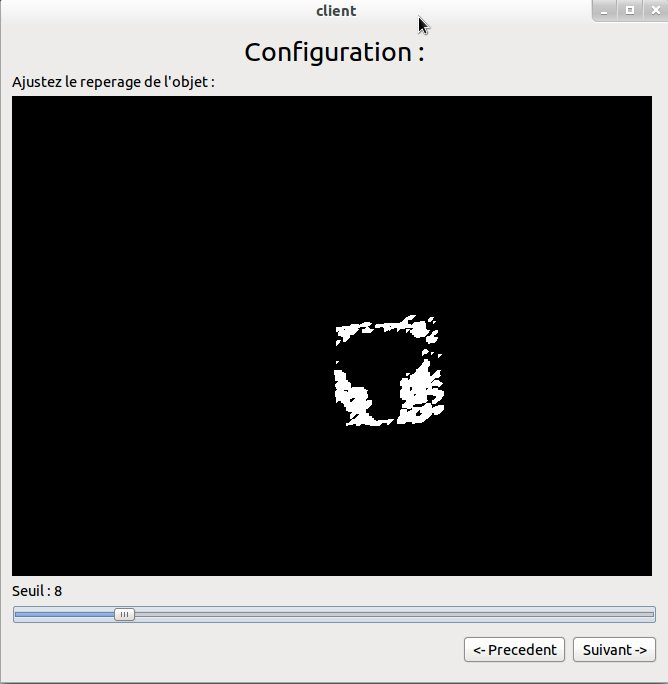
\includegraphics[scale=0.25]{capture1.jpg}
			\end{center}
		\end{frame}

		\begin{frame}{Suivi par couleur : Composante connexe}
			\begin{itemize}
				\item{Calcul des différentes composantes connexes sur l'image binaire}
				\item{Sélection de la composante correspondant au curseur}
				\item{Récupération de son barycentre} 
			\end{itemize}
		\end{frame}

		\subsection{Suivi par Forme}
		\begin{frame}{Étalonnage par forme}
			\begin{itemize}
				\item{Sélection de la zone-objet}
				\item{Création d'une sous-image Template}
			\end{itemize}
		\end{frame}

		\begin{frame}{Suivi par forme}
			\begin{itemize}
				\item{Recherche du template dans l'image}
				\item{Selection de la zone avec la meilleure correspondance}
			\end{itemize}
		\end{frame}
		\subsection{Comparatifs}
		\begin{frame}{Comparatif Couleur/Forme}
		\pause
			\begin{block}{Couleur}
				Avantages \\
				- Traçage rapide \\
				- Diversité possible de curseurs \\
				Faiblesses \\
				- Sensibilité à l'environnement\\
				- Dépendance de la qualité du dispositif d'acquisition\\
			\end{block}
			\pause
			\begin{block}{Forme}
				Avantages \\
				- Traçage moins dépendant de la qualité de l'environnement \\
				- Efficace sur des objets 'complexes'\\
				Faiblesses \\
				- Traçage lent \\
				- Très sensible aux variations du curseur\\
			\end{block}
		\end{frame}
		\begin{frame}{Comparatif Simple/composante connexe}
		\pause
			\begin{block}{Barycentre simple}
				Avantages \\
				- Traçage rapide \\
				Faiblesses \\
				- Sensibilité aux parasites (fausses détections)\\
				- Précision fortement dépendante de l'environnement\\
			\end{block}
			\pause
			\begin{block}{Barycentre composante connexe}
				Avantages \\
				- Traçage plus précis \\
				- Résistance aux parasites \\
				Faiblesses \\
				- Traçage plus lent \\
				- Perte occasionnelle du curseur
			\end{block}
		\end{frame}

		\begin{frame}{Bilan}
			\begin{exampleblock}{Objectifs atteints}
				\begin{itemize}
				\item Librairie utilisable proposant plusieurs solution de traçage
				\item Détection d'action implémentée dans deux des trois solutions
				\item Utilisation simple sans connaissance en traitement des images
				\end{itemize}
			\end{exampleblock}
			\pause
			\begin{alertblock}{Difficultés et ouverture}
				\begin{itemize}
				\item Exploitation des librairies OpenCv et CvBlob 
				\item Implémentation de la détection pour le track par forme
				\item Ajout à la librairie de nouvelles fonctions de track
				\end{itemize}
			\end{alertblock}
		\end{frame}
	
	\section{Application}
		\begin{frame}{Architecture}
			\begin{block}{Objectifs de l'architecture conçue}
				\begin{itemize}
				\item{Avoir une application modulable et facilement extensible}
				\item{Fonctionnement identique pour les classes principales en réseau ou en local}
				\item{Pouvoir rajouter facilement des outils}
				\item{Séparer le traitement du rendu}
				\end{itemize}
			\end{block}
		\end{frame}
		
		\begin{frame}{Diagramme de classes}
			\begin{center}		
			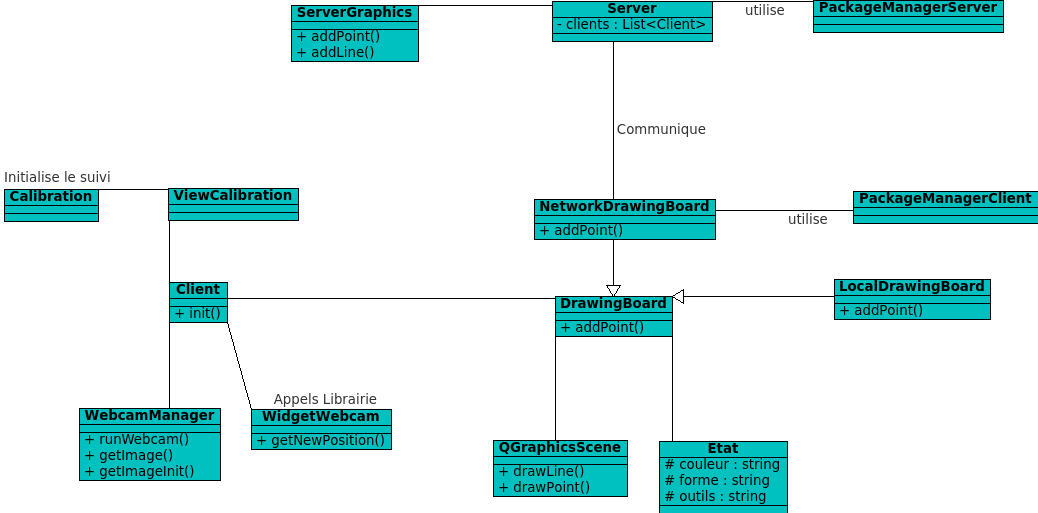
\includegraphics[scale=0.45]{../uml/classes.png}
			\end{center}
		\end{frame}

	\begin{frame}{Application}
			
			L'application est utilisable en local et en réseau, avec un fonctionnement identique.
			
			Les fonctionnalités implémentées sont les suivantes :
			\begin{itemize}
			\item Un outil pour changer la couleur et la forme du pinceau
			\item Un outil gomme
			\item Fonctionnalité permettant d'exporter le dessin
			\item Mode plein-écran avec le dessin uniquement (vidéoprojecteur)
			\item Utilisation simultanée par plusieurs utilisateurs
			\end{itemize}
		\end{frame}
		
	\subsection{Module Local}
		\begin{frame}{Fonctionnemment global}
			\begin{block}{Fonctionnement en local}
				\begin{itemize}
				\item Étalonnage selon la méthode voulue, choix du mode local
				\item Détection d'un mouvement, dessin directement sur le tableau en respectant les options
				\end{itemize}
			\end{block}
		\end{frame}
		
		\begin{frame}{Étalonnage}
			L'étalonnage se déroule en plusieurs phases.
			\begin{itemize}
			\item Choix de la webcam et de méthode de suivi
			\item Choix de l'objet à suivre à partir d'une photo, en l'entourant d'un rectangle
			\item Réglage du seuil de tolérance à partir du retour de l'étalonnage
			\item Choix du mode : réseau ou local
			\end{itemize}
		\end{frame}
		
		% TODO : compléter ou supprimer cette frame
		\begin{frame}{Utilisation de l'application}
		L'interface permets de visualiser le flux vidéo, et le dessin.
		
		Les mouvements sont détectés, et le dessin est effectué à partir de ces mouvements.
		\end{frame}
		
		% Bilan du projet côté interface
		\begin{frame}{Bilan}
			\begin{exampleblock}{Objectifs atteints}
				\begin{itemize}
				\item Application fonctionnelle et utilisable
				\item Beaucoup d'outils voulus implémentés
				\end{itemize}
			\end{exampleblock}
			\pause
			\begin{alertblock}{Difficultés et ouverture}
				\begin{itemize}
				\item Faire une interface gestuelle pour sélectionner gomme, couleur et forme
				\item Améliorer la gestion du dessin
				\item Relancer l'étalonnage sans relancer l'application
				\end{itemize}
			\end{alertblock}
		\end{frame}

	\subsection{Module Reseau}
		\begin{frame}{Fonctionnement global}
			\begin{block}{Fonctionnement en réseau}
				\begin{itemize}
				\item Étalonnage selon la méthode voulue, choix du mode réseau
				\item Récupération du dessin actuel par le client
				\item Détection d'un mouvement
				\item Envoi au serveur de ce mouvement (et des options) en respectant le protocole
				\item Réception du paquet côté serveur, dessin du serveur
				\item Envoi aux clients de ce point, avec les options (épaisseur, couleur)
				\item Réception côté client, et dessin en local
				\end{itemize}
			\end{block}
		\end{frame}
		
		\begin{frame}{Fonctionnemment global : schéma}
		
		Déroulement du fonctionnement en réseau de l'application :
			\begin{center}
			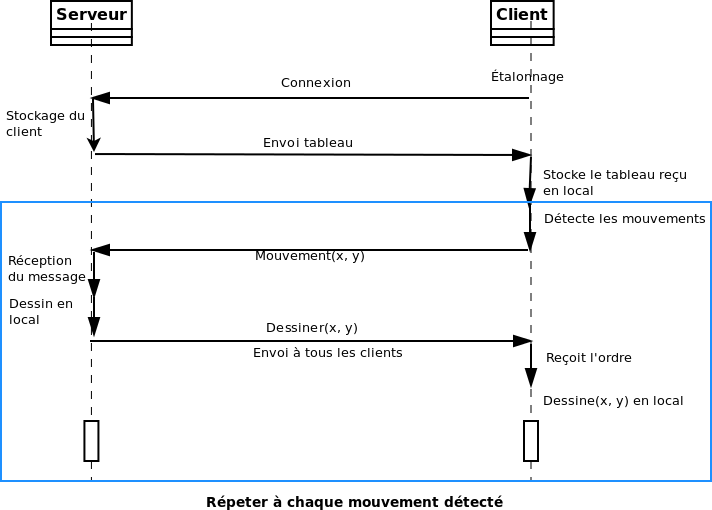
\includegraphics[scale=0.40]{../uml/sequence_reseau.png}
			\end{center}
		\end{frame}
		
		% Bilan de l'application côté réseau
		\begin{frame}{Bilan}
			\begin{exampleblock}{Objectifs atteints}
				\begin{itemize}
				\item Architecture identique au fonctionnement en local
				\item Application fonctionnelle en mode réseau malgré la difficulté
				\item Tous les outils marchent et sont implémentés
				\end{itemize}
			\end{exampleblock}
			\pause
			\begin{alertblock}{Difficultés et ouverture}
				\begin{itemize}
				\item Optimiser fortement le mode réseau pour réduire les problèmes de lenteur
				\item Mettre par défaut une couleur à chaque utilisateur
				\end{itemize}
			\end{alertblock}
		\end{frame}

	\section{Conclusion}
		\begin{frame}{Conclusion}
			\begin{alertblock}{Difficultés}
				- Collaboration : Développement incrémental qui oblige à beaucoup communiquer \\
				- Formation : Traitement de l'image \\
				- Techniques : Architecture, Fuites de mémoire ...\\
			\end{alertblock}
			\pause
			\begin{exampleblock}{Objectifs atteints}
				- Solution fonctionnelle \\
				- Respect du cahier des charges \\
				- Découverte (Objet, Technologies,...) \\ 
			\end{exampleblock}
			\pause
			\begin{block}{Ouverture}
				- Diversifier et optimiser les méthodes de suivi\\
				- Rajouter des fonctionnalités côté application \\
			\end{block}
		\end{frame}
	
	\begin{frame}
		\begin{center}
			\huge{Merci pour votre attention.} \\
		\end{center}
	\end{frame}

\end{document}
